%!TEX root = main.tex

\section{Dataset} \label{sec:dataset}


An important realization we made during this project is the challenge of working with a real dataset.
Understanding the raw data became a significant portion of the project, so this chapter provides a thorough explanation of our findings and methods to process the data.

\subsection{Raw Data}

Our data comes from golf carts equipped with Lidar and cameras~\cite{Miller16_IROS,Miller17_predictive_ICRA}.
Fortunately, it is relatively straightforward to visualize trajectory data, as opposed to some high-dimensional datasets that exist for other applications. 

% what does raw data look like?
The raw dataset's fields are shown in \cref{table_data}, where (easting,northing) are the latitude/longitude global coordinates, and (x,y) are the coordinates in our global campus map.
Veh id indicates which of the three vehicles corresponds to that data point, or in the pedestrian case, which vehicle sensed that pedestrian.
Ped id is a unique id given to each pedestrian seen.

\begin{figure}
	\centering
	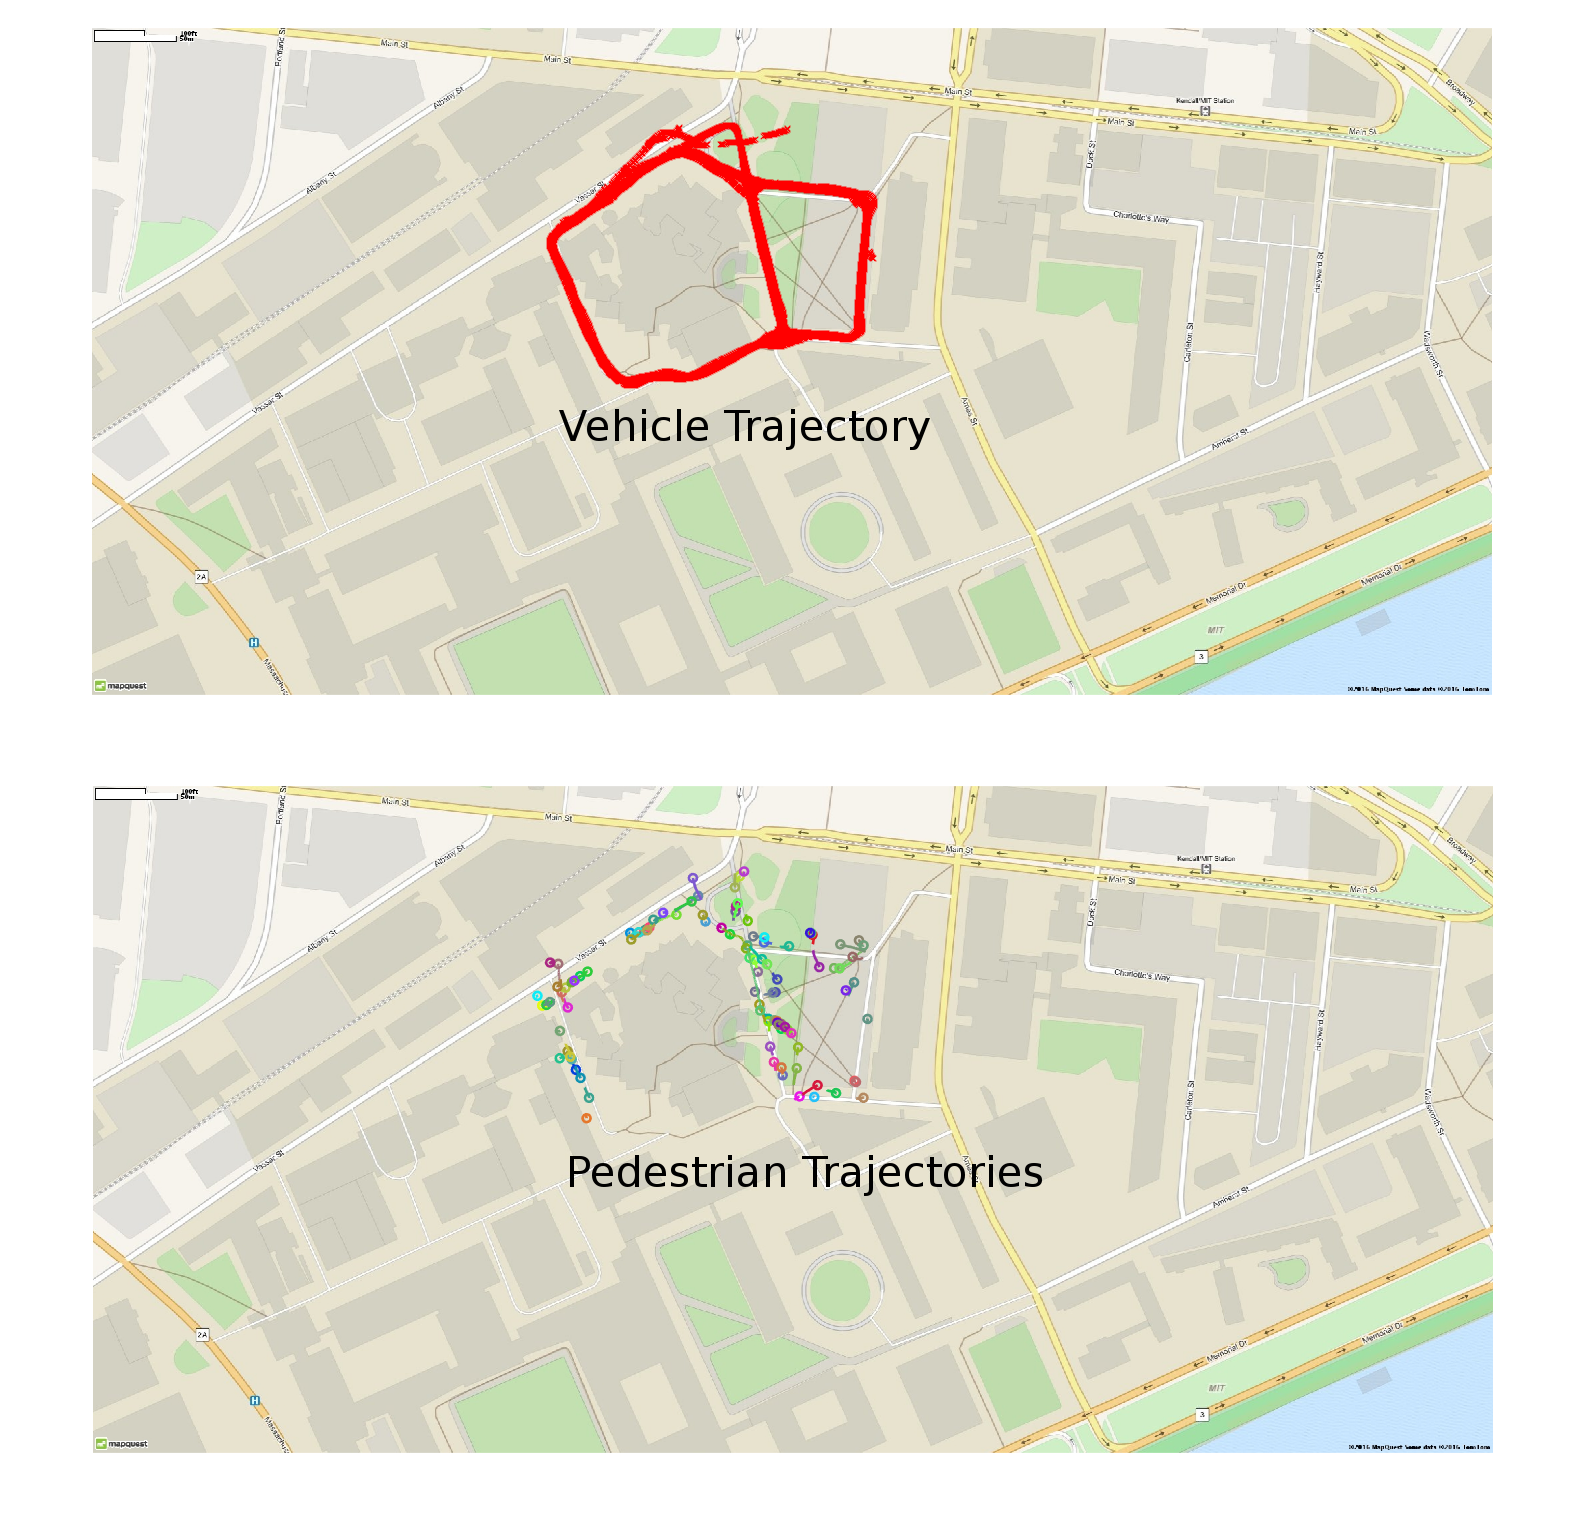
\includegraphics [trim=0 0 0 0, clip, angle=0, width=0.8\columnwidth,
	keepaspectratio]{figures/traj_on_map}
	\caption{The raw trajectories from one day of data collection visualized on a campus map. All trajectories are recorded in the global map coordinate frame.} 
	\label{fig:traj_on_map} 
\end{figure}

\begin{table}[ht!]
\centering
\begin{tabular}{||c||c c c c c c c||}  
 \hline
 \multirow{1}{*}{Type} &
       \multicolumn{7}{c||}{Fields} \\
 \hline\hline
 Vechicle & time & easting & northing & x & y & veh id & \\ \hline
 Pedestrian & time & easting & northing & x & y & veh id & ped id \\ \hline
\end{tabular}
\caption{Raw data fields}
\label{table_data}
\end{table}

% what are the issues with the raw data
There are some noise-related issues with the raw data, as it was collected on a research vehicle under development.
One issue is that the vehicle's (x,y) position sometimes jumps, because the vehicle's localization system does not use GPS and is imperfect.
Other minor issues include pedestrian trajectories that incorrectly split/merge or are too short to be useful for this project.

In addition to addressing noise, we also pre-process the data by converting pedestrian trajectories into the vehicle's local frame.
Our objective is to classify whether pedestrians cross in front of the vehicle, so the pedestrian trajectories must be converted into the vehicle's local frame.
That is, our dataset is initially unlabeled, and we must generate the ground truth label that we wish to learn to classify later.

It might be possible to somehow feed both the vehicle trajectory and pedestrian trajectory into a classifier, and have it learn the transformation, but it seemed much more straightforward for us to rotate the data ahead of time.
Using global coordinates could potentially allow the classifier to learn a global understanding of the map (e.g. where sidewalks/intersections are), but we chose to focus on a more structured problem for this project.
Since global coordinates should have an impact on pedestrian motion, we could in the future try a hybrid approach where we feed local coordinates along with some context features (e.g. distance to curb, traffic light state) as in~\cite{casnsc_NIPS}.

\subsection{Global-to-Local Transformation}

% what is strategy to fix issues
The global-to-local transformation relies on knowledge of vehicle orientation (heading angle) and smooth vehicle trajectories, neither of which we have by default.
\cref{alg:global_to_local} describes the procedure for filtering, transforming, and labeling the raw dataset.

\begin{algorithm}\label{alg:global_to_local}
	\caption{Algorithm for extracting local trajectories}
	\begin{algorithmic}[1]
		\renewcommand{\algorithmicrequire}{\textbf{Input:}}
		\renewcommand{\algorithmicensure}{\textbf{Output:}}
		\REQUIRE $V_g$, $P_g$: global vehicle, pedestrain trajectories~(\cref{table_data})
		\ENSURE  $P_l$: pedestrian trajectories in local vehicle frame
		\FOR {each vehicle}
			\STATE $I_{pos jump}$ = $\{i \in [1,len(V_g)-1] \mid euclid\_dist(V_g(i)-V_g(i+1))>1.0\}$
			\STATE $I_{time jump}$ = $\{i \in [1,len(V_g)-1] \mid time(V_g(i)-V_g(i+1))>0.5\}$
			\STATE J = $I_{pos jump}$ $\cup$ $I_{time jump}$
			\STATE $T_{valid}$ = $\{[J(i), J(i+1)] \mid time(J(i+1) - J(i)) > 5.0\}$
			% \FOR {each segment in $T_{valid}$}
				% \STATE abc
				% \STATE find smooth veh traj
			% % \ENDFOR
			% \FOR {each $P_{g,i}$ pedestrian id}
			% 	\IF {}
			% 		\STATE vxy = 
			% 	\ENDIF
			% \ENDFOR
		\ENDFOR
		\RETURN pedestrian trajectories 
	\end{algorithmic} 
\end{algorithm}

\begin{figure}
	\centering
	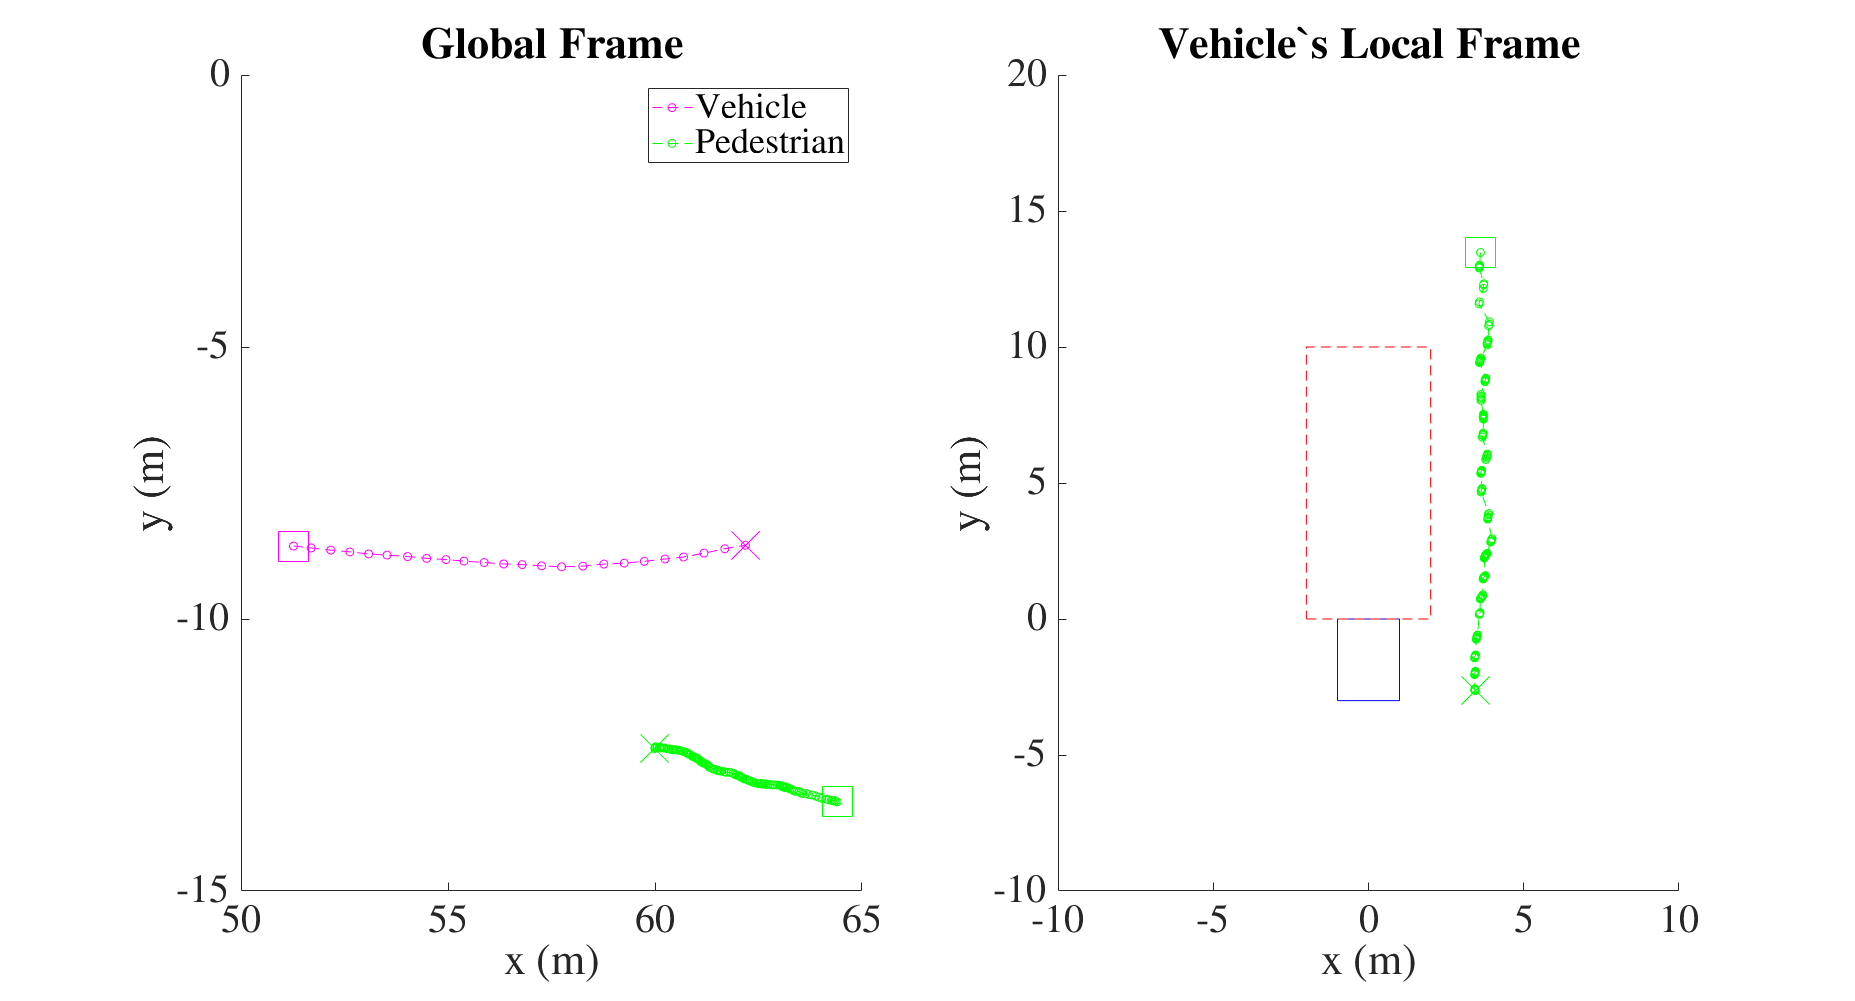
\includegraphics [trim=0 0 0 0, clip, angle=0, width=0.8\columnwidth,
	keepaspectratio]{figures/global_to_local}
	\caption{On the left, the vehicle trajectory (magenta) and pedestrian trajectory (green) in the global frame. Both start from the square and move to the X. On the right is the local vehicle frame: the vehicle is the blue rectangle, and the red dashed rectangle is the ``cross'' zone. The green pedestrian trajectory doesn't cross into the red rectangle, so this trajectory is given binary label 0.} 
	\label{fig:global_to_local_matlab} 
\end{figure}

\subsection{Processed Dataset}

% what does fixed dataset look like
The processed dataset is visualized in~\cref{fig:training_set}.
The vehicle (yellow taxi) has a blue rectangle representing the ``cross'' zone (similar to~\cref{fig:global_to_local_matlab}).
Green trajectories are local pedestrian trajectories that do not cross into the blue zone, and red trajectories are ones that do enter the blue zone.

A few important observations about the processed dataset are the jaggedness and locations of trajectories.
The jaggedness is due to the transformation and sensor rates: the Lidar provides pedestrian trajectory at high rate (50 Hz), but the vehicle position is updated at a slower rate (10 Hz), so the pedestrian trajectory jumps a bit each time vehicle time step.
Since the rotation is dependent on vehicle heading angle, and vehicle heading angle is computed from consecutive vehicle positions, this process is subject to some noise.
It is also somewhat difficult to imagine what local trajectories \textit{should} look like, because these trajectories are showing how the vehicle and pedestrian move relative to one another, and an observer doesn't know what the vehicle's velocity was for any particular trajectory.
For example, a trajectory that arcs along the front of the vehicle could be the vehicle turning as a pedestrian walks straight, or a pedestrian walking in a curve while the vehicle is parked.
All of this could have been avoided if we had access to raw sensor measurements, as these provide local coordinates by default.

The second observation is that the trajectories are in front/along the sides of the vehicle, and have a limited range of about 20m.
This makes sense given our sensor: it is mounted on the vehicle's front and sees a 270$^{\circ}$ cone.
Its maximum range is more than 20m, but tracking pedestrians reliably is difficult beyond this distance.

\begin{figure}
	\centering
	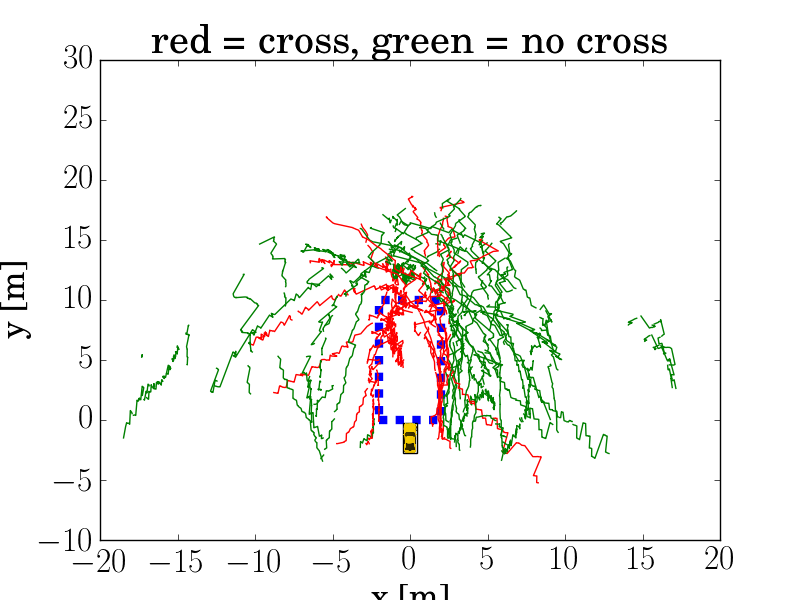
\includegraphics [trim=0 0 0 0, clip, angle=0, width=0.8\columnwidth,
	keepaspectratio]{figures/training_set}
	\caption{A small portion of the training set for the binary classifier. The vehicle (yellow taxi) has a blue rectangle representing the ``cross'' zone. Green trajectories are local pedestrian trajectories that do not cross into the blue zone, and red ones do.} 
	\label{fig:training_set} 
\end{figure}



